\documentclass[conference]{IEEEtran}
\IEEEoverridecommandlockouts
\usepackage{cite}
\usepackage{amsmath,amssymb,amsfonts}
\usepackage{algorithmic}
\usepackage{graphicx}
\usepackage{textcomp}
\usepackage{xcolor}
\usepackage{booktabs}
\usepackage{stfloats}
\graphicspath{{figures/}{./}}
\def\BibTeX{{\rm B\kern-.05em{\sc i\kern-.025em b}\kern-.08em
    T\kern-.1667em\lower.7ex\hbox{E}\kern-.125emX}}
\begin{document}

\title{Quote-Grounded Language Model Context for Football Starting\\Lineup Prediction: Measuring Rather Than Assuming Contamination}

\author{\IEEEauthorblockN{Mohamed Badra}
\IEEEauthorblockA{\textit{Computer Engineering, CAIE Programme} \\
\textit{Ain Shams University, University of East London}\\
Cairo, Egypt \\
mohamedwbadra@gmail.com}
}

\maketitle

\begin{center}
\vspace{-4mm}
\footnotesize
Code and extracted signals: \texttt{https://github.com/mwbadra/quote-grounded-lineup-prediction}
\vspace{2mm}
\end{center}

\begin{abstract}
Predicting a football manager's starting eleven before kick-off is difficult because the decisive information --- injuries, rest and internal competition --- appears in natural language rather than in structured databases. This paper fuses tabular match data with contextual signals extracted from pre-match reporting by a large language model (LLM), evaluated on the complete 2025--2026 English Premier League season: 740 team-matches and 20{,}287 player-match observations with confirmed team sheets as labels. The pipeline identifies nine or more of the eleven starters in $70.3\%$ of validation squads, against $56.4\%$ for the strongest no-model recency rule passed through the identical assignment stage, and attains $80.89\%$ constrained lineup accuracy. Two design decisions distinguish the study: the candidate pool is the club's \emph{available} squad, a mean of 27.4 players reconstructed from per-gameweek availability snapshots rather than the announced matchday squad of roughly twenty; and every extracted signal must cite a verbatim span verified against the retrieved text in code, so that a signal recalled rather than read is discarded. The pooled contribution of the contextual block is small, $+0.0008$ in accuracy and a significant $+0.0040$ in ROC-AUC, and we argue this is the expected result rather than a disappointing one: selection is governed by ability and recent participation, which the tabular block already encodes, leaving language only the residual of decisions driven by injury, rest and managerial intent. The effect is therefore properly read at squad level, where the contextual block is worth $+2.5$ points at nine-of-eleven, and on the $7.23\%$ of rows the signal actually reaches, where it lifts ROC-AUC by $+0.0363$ ($95\%$ CI $[+0.019, +0.053]$), nine times the pooled gain. A three-arm ablation then measures rather than assumes contamination. Prompted with no sources the same model reaches ROC-AUC $0.654$ on $68.4\%$ of player-matches; but on the cases where both conditions speak, the unsourced signal falls to $0.513$, indistinguishable from chance, against $0.713$ for the quote-grounded one, agreeing only $34.1\%$ of the time. We further report three negative results, on formation forecasting, positional partitioning and richer encodings of the LLM output.
\end{abstract}

\begin{IEEEkeywords}
Football analytics, starting lineup prediction, large language models, retrieval grounding, data contamination, gradient boosting, assignment problem, English Premier League
\end{IEEEkeywords}

\section{Introduction}

Association football is tactically more complex than team-level statistics can capture, and at the centre of that complexity sits the manager's team selection. This decision, typically finalised hours before kick-off, is shaped by recent form, accumulated fatigue, injury status, tactical counter-planning and managerial preference. Many of these signals reach the public through press conferences, injury bulletins and beat journalism rather than through structured statistical feeds.

The value of predicting that decision is substantial. Fantasy football platforms engage millions of participants, each selecting a personal eleven before every deadline; the official Fantasy Premier League alone engaged over 11 million users in 2025 \cite{ramezanidinh2025}. Broadcasters, scouting departments and club analytics teams depend increasingly on computational decision support. Despite this, automated lineup prediction remains underdeveloped relative to match outcome and score forecasting.

The dominant paradigm employs structured statistical features such as Elo ratings, cumulative season metrics and positional indices as inputs to classifiers or regressors \cite{hvattumarntzen2010, debdas2026, peterspacheco2023}. These approaches are methodologically rigorous but architecturally blind to the pre-match contextual information on which managers themselves act. An emerging strand explores text-derived features, principally social media sentiment, as augmentations to match prediction \cite{wunderlichmemmert2022}; these operate at team level on aggregate sentiment rather than at the level of the individual selection decision.

Applying an LLM here introduces a difficulty the sports analytics literature has largely left unaddressed. Any model trained after a season concluded may simply \emph{recall} its team sheets, and a claimed knowledge cutoff does not resolve this, because cutoffs are approximate and a reader cannot verify one. The contribution is therefore as much methodological as empirical: contamination is structurally constrained and then measured rather than assumed away.

The contributions are as follows:

\begin{enumerate}
    \item[(i)] A \emph{quote-grounded} extraction procedure in which every contextual signal must cite a verbatim span verified against the retrieved text in code, so that recalled assertions are discarded rather than trusted.
    \item[(ii)] A three-arm contamination ablation, comprising sourced, memory-only and shuffled-source conditions, that measures how much of the signal is read and how much is recalled.
    \item[(iii)] An evaluation protocol using confirmed team sheets, an availability-derived candidate pool of 27.4 players, and a no-model baseline passed through the identical assignment stage.
    \item[(iv)] Position-relative percentile features that encode competition for a place, together with three negative results concerning formation forecasting, positional partitioning and LLM output encoding.
\end{enumerate}

Section II reviews related work, Section III the method, Section IV the evaluation, and Sections V and VI the findings and limitations.

\section{Related Work}

\subsection{Football Match Outcome Prediction}

Prediction of football outcomes has attracted sustained attention since Maher's Poisson model for goal scoring \cite{maher1982}. Hvattum and Arntzen derived Elo covariates for ordered logit models and evaluated them against six benchmarks under statistical and economic criteria \cite{hvattumarntzen2010}; Horvat and Job review over twenty models and confirm that classification consistently outperforms regression on this task \cite{horvatjob2020}. Most relevant here, Peters and Pacheco showed on 2020--2022 Premier League data that goalkeeper statistics exert disproportionate influence, and that supplying the announced lineup, encoded as season-to-date statistics averaged within each position group, does not materially improve score prediction \cite{peterspacheco2023}. That result distinguishes player \emph{presence} from player \emph{contextual state}: an aggregate of a player's past output carries no information about whether he is rested, doubtful or out of favour this week.

\subsection{Lineup Selection and Team Composition}

A separate strand treats lineup selection as discrete optimisation. Deb and Das combine LASSO-induced multinomial logistic regression over player combinations with a GRASP meta-heuristic \cite{debdas2026}, and Ramezani and Dinh formulate fantasy team selection as deterministic and robust mixed-integer programs subject to budget, formation and club-quota constraints \cite{ramezanidinh2025}. Both are prescriptive, identifying which lineup \emph{would have} maximised a known objective, whereas the present work must forecast a human decision for which no such function exists; the positional eligibility structure considered here also reduces to bipartite assignment and is solvable exactly in polynomial time.

Cortez et al. address the line-up question directly, deriving a preparedness index by applying recursive feature elimination and logistic regression to 16{,}996 GPS player-session episodes from a single club \cite{cortez2022}. It yields usable models for only three outfield positions, excludes goalkeepers, and depends on proprietary telemetry; the dataset used here exposes comparable physical-load measures for all twenty clubs. Hirotsu and Wright applied Markov processes to formation and substitution strategy \cite{hirotsuwright2003}, which motivated the formation forecasting module we evaluate and, as Section IV-D reports, discard. Cao et al. observe that fully automated lineup models are seldom adopted in professional practice precisely because they omit the coach's judgement \cite{caoetal2022}, which motivates treating managerial signals as an explicit input.

\subsection{Language Models in Sports Analytics}

Caron and M\"uller fine-tune a foundation model with low-rank adapters on 100{,}000 textual sequences derived from 580 Premier League fixtures \cite{caronmueller2023}. On questions requiring the model to name the player involved in a situation, only $32\%$ of responses were judged factually correct although $62\%$ were judged plausible, so direct generative identification of individuals is unreliable even for a domain-adapted model. That motivates the division of labour adopted here, in which the language model extracts bounded contextual labels rather than naming players and the player-level decision is delegated to a constrained tabular classifier. Horton and Lucey establish that attention-based architectures can represent interactions between player ability and evolving context, though for in-game rather than pre-match forecasting \cite{hortonlucey2025}.

Wunderlich and Memmert applied sentiment analysis to almost two million tweets from more than 400 Premier League matches and found that in-play information does not improve forecasting accuracy relative to pre-game information \cite{wunderlichmemmert2022}, motivating the present focus on the pre-match window. Schr\"oder et al. benchmark seven language models on prospective match forecasts and find that web access reduces mean Brier score from $0.535$ to $0.512$ ($p = 0.045$), with a human audit showing web-enabled models reference injuries or lineups $53.0$ percentage points more often \cite{schroeder2026}. This is independent evidence that pre-match natural language carries retrievable signal concerning availability and rotation.

No prior work, however, targets the player-level starting decision using publicly retrievable pre-match text with an explicit, verifiable control against the language model recalling the evaluation period from its training data. That control is the central methodological contribution here.

\section{Method}

\subsection{Problem Statement}

Let $p$ denote a player in the available squad $A^{c}_{m}$ of club $c$ for fixture $m$. We define the binary target
\begin{equation}
y_{pm} =
\begin{cases}
1, & \text{if player } p \text{ starts match } m, \\
0, & \text{otherwise,}
\end{cases}
\label{eq:target}
\end{equation}
and, given a feature vector $x_{pm}$ constructed exclusively from information available strictly before kick-off, estimate
\begin{equation}
P\left(y_{pm} = 1 \mid x_{pm}\right),
\label{eq:posterior}
\end{equation}
subsequently resolving the estimates into a positionally coherent eleven $L^{c}_{m} \subset A^{c}_{m}$ with $|L^{c}_{m}| = 11$.

\subsection{Tools and Models}

Four components carry the pipeline, each chosen for one specific property. Retrieval uses \textbf{Tavily}, which accepts an explicit publication-date range, closed here the day before kick-off, and returns cleaned article text rather than raw pages. The bound is enforced at the request; per-article publication dates are not retained in the corpus. Extraction uses \textbf{Gemini 3.1 Flash Lite}. A small model suffices because the task is bounded: it never predicts a lineup or reasons about tactics, but reads a passage, copies the relevant sentence and picks one label from a closed list, returning mechanically validated JSON. This avoids the regime in which Caron and M\"uller found open-ended generative identification unreliable \cite{caronmueller2023}, and keeps roughly 1{,}200 calls affordable. \textbf{XGBoost} \cite{chenguestrin2016} estimates the starting probability, chosen because it handles missing values natively --- roughly ninety per cent of the contextual features are absent by construction and no imputation would be honest --- and splits on an integer-coded position label, so a tree may condition on position at the root while still pooling across positions, a property Section V-D shows to matter. \textbf{The Hungarian algorithm} \cite{kuhn1955} resolves the final eleven in polynomial time, so any error is attributable to the probability estimates rather than the search.

\subsection{Stage 0/1: Data and the Candidate Pool}

Data are retrieved programmatically from the season-partitioned endpoints of \texttt{FPL-Core-Insights} \cite{fpleloinsights}, itself derived from the official Fantasy Premier League API \cite{fplapi}. The evaluation covers gameweeks 2 to 38 of the 2025--2026 Premier League: 370 fixtures, 740 team-matches and 20{,}287 player-match observations. Three tables carry the design. A per-gameweek \texttt{lineups} table supplies the label as an observed boolean starting flag, which resolves to exactly eleven players for all 740 team-matches, so no selection has to be inferred from minutes played. Per-gameweek player status snapshots supply the candidate pool. Average on-pitch coordinates supply the position taxonomy.

The candidate pool for fixture $m$ comprises every registered player whose status in the gameweek $N-1$ snapshot is \emph{available} or \emph{doubtful}, giving a mean of 27.4 players per team-match. Reading availability from the preceding snapshot is deliberately conservative: it withholds any status change in the final days before kick-off, supplying the model with strictly less information than a forecaster would possess. The cost is small and measurable, $99.42\%$ of actual starters being present in their pool, and we state the direction of the residual bias rather than leave it implicit. At row level the omission is a pure penalty, since a starter outside the pool can never be recovered. At squad level it is not, because a team-match whose pool is missing a starter cannot reach eleven correct and is excluded from the squad metrics rather than scored as a failure. This affects 39 of the 740 team-matches across the season but only 2 of the 238 in validation, which is why squad results below are reported on 236 squads; scoring those two moves nine-of-eleven by at most $0.6$ points either way.

Player positions are derived from average on-pitch coordinates in prior matches, reduced to seven coarse slots: goalkeeper, plus centre and wide for each of defence, midfield and attack. Positional purity --- the share of a player's appearances at his modal slot, over players with at least ten appearances --- is $0.841$ under this scheme. A finer taxonomy separating left from right was rejected because full-backs and wingers exchange flanks routinely, fragmenting a player's history across two labels.

\subsection{Stage 2: Quote-Grounded Contextual Extraction}

For each team-match, retrieval covers a window opening five days before kick-off and closing the day before, clamped so that it never reaches back past the club's previous fixture. Results are scored for pre-match relevance, where preview and press-conference language raises the score while report language and scorelines eliminate it. Articles whose title names both clubs are attributed by counting mentions of each squad, since such a title cannot by itself establish which club the article concerns.

A single language model call per team-match returns, for each discussed player, a rotation label drawn from a closed set and an optional sentiment label, together with a supporting quote and a declared source type. Two constraints are then enforced in code rather than in the prompt:

\begin{enumerate}
    \item[(a)] \textbf{Quote grounding.} The quoted span must appear verbatim in the retrieved text after whitespace, punctuation and accent normalisation. Spans failing this check are discarded, as are spans shorter than a length floor unless they name a squad member.
    \item[(b)] \textbf{Source typing.} Signals declared as fantasy-football advice are rejected outright, and signals declared as journalistic prediction are demoted from \emph{explicit} to \emph{implied}.
\end{enumerate}

Grounding serves two purposes at once. It is a hallucination control, and the first line of the contamination control, because an assertion recalled from training data cannot be paired with a span occurring in the retrieved articles. It constrains rather than eliminates the recall route, since the model still chooses which spans to surface; Section IV-E measures what is left. Of 1{,}643 candidate signals, 1{,}567 were accepted and 76 rejected ($4.6\%$): 59 for insufficient span length and 17 because the quoted text did not occur in the sources.

The extraction stage distinguishes four outcomes rather than collapsing them: a signal was found, the sources were read and said nothing about this player, no source passed the relevance filter, or the call failed. There were no failed calls at either stage. Only the second is a genuine negative; the third is missing data and accounts for $32\%$ of fixtures (Section VI). The modelling table carries a single null for all three non-signal states, so the distinction survives in the extraction record but is not exposed to the classifier --- an encoding that recovers it was tested and did not help (Section V-D).

\subsection{Stage 3: Probability Model and Position-Relative Features}

Starting probabilities are estimated over three feature blocks: seventeen tabular features spanning selection history, availability, defensive and attacking output and discipline; a twelve-column \emph{position-relative} block, being eleven percentile transforms plus a count of how many rivals the player has at his position in that squad; and the language model signals.

The percentile block replaces a raw statistic with the player's rank among players of his own position group within his own available squad for that fixture. The selection logic motivates it: a manager picks the best available centre-back, not every centre-back above an absolute threshold, so rank among rivals for the shirt is the selection-relevant quantity and the raw value cannot express it. Empirically the percentile transform strengthens the association with the target for nine of eleven statistics, most sharply for defensive actions ($|r| = 0.395$ rising to $0.588$) and recoveries ($0.463$ rising to $0.612$).

Monotone constraints on the seven features carrying an unambiguous directional prior --- \texttt{start\_rate\_last\_5}, \texttt{consecutive\_starts}, their two percentile transforms and \texttt{availability\_score} increasing, the player- and team-level rotation signals decreasing --- were evaluated and \emph{not} adopted. Constraining only the two raw recency columns understates the cost, because the unconstrained percentile copies then carry the same information. Imposing all seven costs $0.42$ percentage points of constrained lineup accuracy and $3.0$ points at nine-of-eleven, which indicates that the unconstrained fit already respects those priors and that the constraint only removes capacity. The discrimination cost is small in relative terms, $0.10\%$ of ROC-AUC, which sits inside the range Koklev reports for monotone-constrained gradient boosting on credit data, from essentially zero on large samples to roughly $2.9\%$ on smaller ones carrying extensive constraint coverage \cite{koklev2025}. What decided the matter is the squad-level cost, not the row-level one: the assignment stage consumes the ranking, and a constrained ranking loses nine-of-eleven lineups. The preliminary system applied such constraints; the present one does not, and every figure below is from an unconstrained fit.

\subsection{Stage 4: Positional Assignment}

Taking the eleven highest probabilities is not an admissible output, whatever it scores: the classifier is fitted per player and knows nothing of the joint constraint, so nothing stops it returning two goalkeepers or none. Stage 4 exists to make every output a legal eleven, and the metric is defined only over legal elevens. The formation is mapped to an eleven-slot template whose composition is learned from the data, taking for each formation string the modal composition of coarse slots among observed starters. The Hungarian algorithm then solves
\begin{equation}
\hat{\pi} = \arg\max_{\pi \in \Pi} \sum_{k=1}^{11} P\left(\text{starter} \mid x_{\pi(k),m}\right)
\label{eq:hungarian}
\end{equation}
subject to positional eligibility. Eligibility is deliberately permissive across the wide and centre boundary within a line, and one line adjacent, reflecting movement observed in the coordinate data.

\section{Experimental Evaluation}

All experiments use a chronological split at gameweek 27, giving 13{,}746 training and 6{,}541 validation observations across 238 validation team-matches, of which 236 carry their full complement of eleven starters inside the candidate pool and therefore enter the squad-level metrics (Section III-C). Unless stated otherwise, a model is fitted under five random seeds and scored on the mean of the five predicted probability vectors, which is also the vector the assignment stage consumes, so the row-level and squad-level figures in a given table row describe the same object. The one exception, the architecture comparison in Section IV-C, is noted where it appears. Reported dispersions are standard deviations across folds or seeds as indicated.

\subsection{Feature Contribution}

\begin{table}[!t]
\centering
\small
\caption{Feature ablation, chronological split, five seeds}
\label{tab:ablation}
\begin{tabular}{@{}lccc@{}}
\toprule
\textbf{Configuration} & \textbf{Acc.} & \textbf{ROC-AUC} & \textbf{$\geq$9/11} \\
\midrule
Tabular (17 features)          & 0.8372 & 0.9168 & 63.6\% \\
$+$ position percentiles       & 0.8454 & 0.9180 & 67.8\% \\
$+$ LLM signals (proposed)     & \textbf{0.8462} & \textbf{0.9220} & \textbf{70.3\%} \\
\bottomrule
\end{tabular}
\end{table}

Table~\ref{tab:ablation} reports the ablation. Each increment is measured against the strongest preceding configuration rather than a reduced one, since the apparent contribution of any feature group rises as the baseline is weakened, an effect quantified below.

The largest increment the language model produces is the squad-level one: nine-of-eleven rises $2.5$ percentage points, from $67.8\%$ to $70.3\%$. At row level the same features are worth $+0.0008$ in accuracy and $+0.0040$ in ROC-AUC. A paired McNemar test on the accuracy difference is not significant ($\chi^{2} = 0.130$, $p = 0.72$), and a bootstrap over 2{,}000 resamples places it at $[-0.0024, +0.0038]$, including zero; the ROC-AUC difference is $[+0.0028, +0.0052]$, excluding it, and survives a cluster bootstrap over the 238 team-matches at $[+0.0026, +0.0055]$. Since exactly eleven of some twenty-seven candidates start, rows within a squad are not independent and the clustered interval is the one to read. The honest statement is therefore that the contextual signals improve the \emph{ranking} of candidates but not row-level classification, which is precisely why the squad-level effect is the larger of the two: Stage 4 consumes the ranking rather than a decision threshold.

Taken on its own the contextual rotation label correlates with the starting indicator at $-0.446$, comparable to the strongest tabular features, but on only 1{,}466 of the 20{,}287 rows against their full coverage. The two are therefore not like for like, and the marginal correlation of a sparse feature should not be read as its contribution to the pipeline. Restricting to the $10.7\%$ of validation rows that carry a signal, ROC-AUC rises from $0.7312$ to $0.7675$ on those 702 rows, a gain of $+0.0363$ with a bootstrap interval of $[+0.0193, +0.0526]$ and nine times the pooled figure. We deliberately do not quote the accuracy increment on this subset: it is $+0.0085$, but that is a net six rows and its own paired test does not reject ($p = 0.59$), so reporting it as an effect would apply a weaker standard of evidence to the favourable number than to the pooled one. The feature is sparse, and where present it reorders rather than reclassifies.

\subsection{Baseline Dependence of the Reported Increment}

\begin{table}[!t]
\centering
\small
\caption{The same LLM features against three baselines}
\label{tab:baseline_dep}
\begin{tabular}{@{}lcc@{}}
\toprule
\textbf{Baseline} & \textbf{$\Delta$ Acc.} & \textbf{$\Delta$ ROC-AUC} \\
\midrule
Recency only (2 features)      & $+0.0083$ & $+0.0136$ \\
Without recency (15 features)  & $+0.0035$ & $+0.0038$ \\
Full tabular $+$ percentiles   & $+0.0008$ & $+0.0040$ \\
\bottomrule
\end{tabular}
\end{table}

Table~\ref{tab:baseline_dep} applies the identical language model features to three baselines of differing strength. The apparent increment varies by a factor of ten. We report the last row as the headline because it is measured against the strongest model we possess, and include the first so the reader can calibrate published increments of this kind. The point is not hypothetical: a preliminary version of this system reported a $+0.0715$ accuracy increment for the same contextual dimensions against a two-feature comparator, which the first row shows to be an artefact of the baseline rather than a property of the signal.

\subsection{Stability and Baselines}

\begin{table}[!t]
\centering
\small
\caption{No-model baselines through the identical Stage 4}
\label{tab:baselines}
\begin{tabular}{@{}lcc@{}}
\toprule
\textbf{Ranking rule} & \textbf{Constrained} & \textbf{$\geq$9/11} \\
\midrule
Random                       & 41.41\% & 0.4\% \\
Availability only            & 48.04\% & 0.8\% \\
Recent start rate only       & 75.81\% & 52.1\% \\
Consecutive starts only      & 76.31\% & 56.4\% \\
\midrule
Full pipeline                & \textbf{80.89\%} & \textbf{70.3\%} \\
\bottomrule
\end{tabular}
\end{table}

Five forward-chaining folds give mean accuracy $0.8489 \pm 0.0100$, ROC-AUC $0.9252 \pm 0.0079$ and constrained lineup accuracy $81.11\% \pm 1.76$. Performance is stable across the first four folds and degrades in the final block covering gameweeks 34 to 38 ($77.61\%$ constrained, $60.0\%$ at nine-of-eleven), consistent with elevated rotation once league objectives are settled. Fig.~\ref{fig:cv} shows the trajectory.

Table~\ref{tab:baselines} reports baselines that bypass the model entirely, ranking players by a single feature and passing the result through the same assignment stage. Random scoring recovers $41.41\%$, the floor imposed by the assignment constraints alone. We measure the pipeline against the \emph{strongest} of these rules rather than the most convenient one, in the abstract as well as here: consecutive starts reaches $76.31\%$ constrained accuracy and $56.4\%$ at nine-of-eleven, and the full pipeline improves on it by $4.58$ and $13.9$ points. Against recent start rate, the weaker recency rule, the same gaps read $5.08$ and $18.2$ --- a third larger on the second measure for no reason but the choice of comparator, which is the calibration Section IV-B asks the reader to apply. The nine-of-eleven gap is the more meaningful, since that threshold corresponds to a lineup usable in practice, and it is roughly three times the gap on mean accuracy.

A separate comparison across four classifiers on identical features and split places accuracy within a span of $0.0054$, from $0.8390$ for logistic regression to $0.8444$ for random forest with the proposed model at $0.8436$. Because logistic regression and random forests cannot consume missing values, that comparison substitutes a sentinel in all four arms and uses a single seed, so only the spread between architectures should be read from it. That spread indicates the ceiling is set by the information content of the feature space, not by model capacity. The proposed model is retained because it alone consumes the contextual block in its natural form, as a value genuinely absent rather than imputed.

\begin{figure}[!t]
\centering
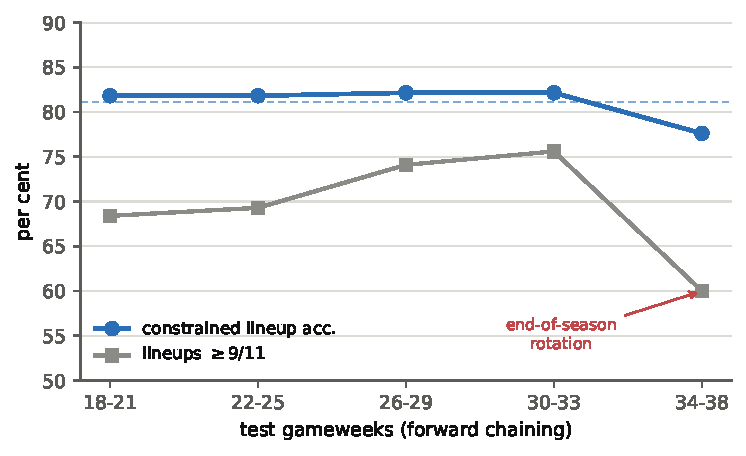
\includegraphics[width=\linewidth]{fig4_cv_stability.pdf}
\caption{Forward-chaining cross-validation. Each fold trains on all gameweeks preceding its test block. The final block degrades as clubs with settled objectives rotate heavily.}
\label{fig:cv}
\end{figure}

\subsection{Formation Forecasting Has No Effect}

All figures here are computed on the proposed configuration. A first-order Markov chain over each club's formation history predicts the fielded shape correctly on $69.9\%$ of the 236 validation squads, marginally below a recency heuristic that reuses the previous formation at $70.3\%$. More consequentially, supplying the \emph{true} formation as an oracle buys almost nothing: $81.01\%$ constrained lineup accuracy against $80.89\%$ under the Markov forecast and $80.93\%$ under recency, a spread of $0.12$ points (Fig.~\ref{fig:formation}). On the 71 squads where the forecast is wrong --- the only ones on which the conditions can differ --- the oracle recovers $8.52$ of eleven starters against $8.48$; on the 36 whose template differs by two or more slots, $8.39$ against $8.33$. The two conditions select the \emph{same eleven players} in 208 of the 236 squads. The decisive control removes formation from the problem altogether: a single constant shape imposed on every fixture gives $80.89\%$ and $72.0\%$ at nine-of-eleven, matching the forecast on the first measure and beating it on the second, and only a randomly drawn formation degrades the result, to $80.64\%$ averaged over twenty draws.

The mechanism is the eligibility graph. A player eligible for a central midfield slot is also eligible for a wide one, and a wide defender covers a central defensive slot, so exchanging one slot for another changes which slot a player fills but not which eleven are chosen. Formation determines the labelling, not the selection, and the stage is accordingly removed from the pipeline. The result is conditional on the coarse taxonomy of Section III-C, since a finer one would bind more tightly, at the cost of the positional instability documented there.

\begin{figure}[!t]
\centering
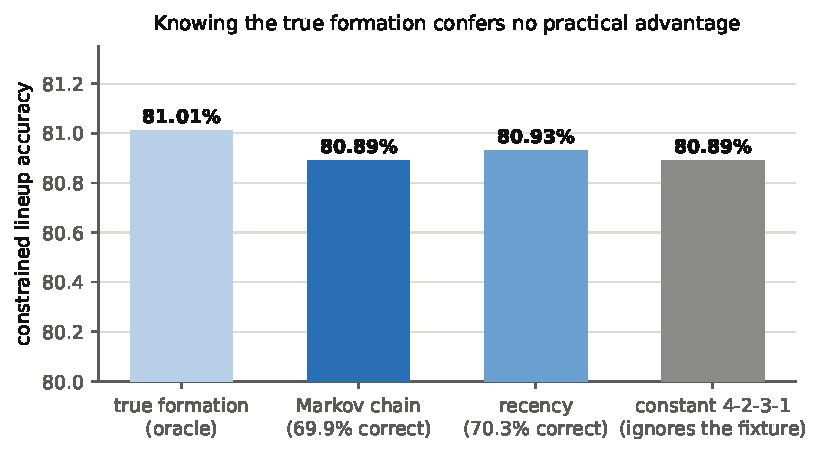
\includegraphics[width=\linewidth]{fig7_formation_conditions.pdf}
\caption{Constrained lineup accuracy under four formation conditions, on the proposed configuration. Supplying the true formation confers no practical advantage, and a single constant shape imposed on every fixture matches the forecast.}
\label{fig:formation}
\end{figure}

\subsection{Contamination Ablation}

\begin{table}[!t]
\centering
\small
\caption{Contamination ablation, validation window. Coverage and ROC-AUC are
computed on each arm's own covered rows and are therefore not directly
comparable across arms; the matched comparison is given in the text.}
\label{tab:leakage}
\begin{tabular}{@{}lccc@{}}
\toprule
\textbf{Arm} & \textbf{Coverage} & \textbf{ROC-AUC} & \textbf{$n$} \\
\midrule
A\; Sourced, quotes verified & 10.7\% & \textbf{0.711} & 702 \\
B\; Memory only, no sources  & 68.4\% & 0.654 & 4{,}477 \\
C\; Shuffled sources         & 1.5\%  & 0.598 & 97 \\
\bottomrule
\end{tabular}
\end{table}

The language model used here was trained after the evaluation season concluded, so the possibility that it recalls team sheets rather than reading them must be addressed empirically. Three arms were run over the same rosters, varying what the model was given to work from (Table~\ref{tab:leakage}). Two asymmetries are stated at the outset. The memory arm is necessarily prompted differently, since a quote requirement would zero its output by construction, and is instead asked for a direct judgement; coverage across arms is therefore not a controlled contrast and we draw no inference from it. The shuffled arm also covers fewer fixtures, 178 of the 238, because it requires a second club in the same gameweek to have a usable corpus to borrow.

Arm B establishes that the model possesses substantial parametric knowledge of the evaluation season. Given only the club, date, opponent and roster, it volunteers a judgement on $68.4\%$ of player-matches and attains ROC-AUC $0.654$ against a chance level of $0.5$. This is a real contamination risk and we report it as such.

The inference that matters is therefore drawn on the 604 player-matches where the sourced and unsourced arms both speak, which is the only population on which the two are comparable. There the unsourced signal collapses to ROC-AUC $0.513$, statistically indistinguishable from chance, while the quote-grounded signal holds at $0.713$. On the same 604 cases the two arms agree on only $34.1\%$; were the grounded signal a repackaging of recall, agreement would be high and the two discrimination figures would converge. Instead the grounded signal separates starters from non-starters on exactly the cases where unaided recall does not.

The shuffled-source control survives on $1.5\%$ of rows, confirming that verification against the wrong club's text eliminates almost all output and that the pipeline is not pattern-matching prompt structure; at $n = 97$ its ROC-AUC of $0.598$ carries little precision and we rest the control on the coverage collapse. The verification gate is itself a modest filter, rejecting $4.6\%$ of candidate signals; what restricts the contextual block to a small share of rows is retrieval coverage (Section VI), not the gate.

The residual limitation is plain: grounding constrains what the model may assert, but it still chooses which spans to surface and which labels to attach, with its parametric knowledge intact. The ablation bounds contamination; it does not eliminate it.

\subsection{Squad-Level Results}

The proposed configuration reaches nine or more correct starters in $70.3\%$ of the 236 validation squads, the operationally meaningful outcome, and attains $80.89\%$ constrained lineup accuracy. Sixteen squads ($6.8\%$) are predicted exactly, 67 at ten and 83 at nine, and the lower tail is short: only 11 of 236 fall below seven correct.

\section{Discussion}

\subsection{Why a Small Pooled Effect Is the Expected Result}

The contextual increment is small, and it should be. Team selection is overwhelmingly determined by two things a structured feed already records: how good a player is, and whether he has been playing recently. Recent start rate correlates with the starting indicator at $+0.687$, and the four selection-history columns carry $63.0\%$ of the fitted model's gain against $1.24\%$ for the contextual label (single fit, seed 42; the split moves a few points across seeds). A manager naming an eleven is, for most of the sheet, confirming what the previous eleven already implied. That regularity is what makes the task learnable at all, and it is also what caps the headroom available to any further source of evidence.

What the tabular block cannot see is the residual: the decision that departs from the pattern because of information generated in the days before kick-off --- an injury in training, a rest ahead of a congested week, a player out of favour, a manager who has said what he intends to do. These reach the public as language rather than numbers, and are irreducibly a minority of selections, so a feature addressing them cannot move a pooled average dominated by decisions that were never in doubt. Judging it by that average understates it by construction. Three measurements agree with the account: the signal reaches only $7.23\%$ of rows; on those rows it lifts ROC-AUC by $+0.0363$, nine times the pooled gain; and the effect it produces is a reordering rather than a reclassification, worth $2.5$ points at nine-of-eleven and nothing detectable at the $0.5$ threshold, which is exactly what reshuffling a handful of contested places within a squad would look like.

\subsection{What the Contextual Signals Capture}

An error analysis of the tabular model locates its failures precisely. Sixty-nine per cent of errors involve players whose recent start rate lies strictly between zero and one, the rotation middle ground; players who started none or all of their recent matches are classified at $4.3\%$ and $13.3\%$ error. Within the errors, $19.8\%$ are established regulars rested and $10.2\%$ fringe players recalled. Only $0.1\%$ involve players new to the league, a category we expected to matter and which the data shows does not.

The extracted signals target exactly this population. Players labelled \emph{confirmed starter} start $81.8\%$ of the time ($n = 33$), \emph{expected starter} $72.0\%$ ($n = 661$), \emph{rotation risk} $32.9\%$ ($n = 641$) and \emph{ruled out} $10.1\%$ ($n = 119$). The comparator for these rates is $49.7\%$, the base rate among the rows that carry a signal, and not the $39.9\%$ that holds across all rows: reporting against the latter would credit the labels with a separation that is partly just the tendency of pre-match copy to discuss first-team players. The ordering is monotone in the four populated labels. The fifth, \emph{competition lost}, fires on twelve rows at a start rate of $16.7\%$ and sits out of order relative to \emph{rotation risk}; at that sample size we treat it as noise, but we report it rather than omit the label that does not fit.

\subsection{Why the Sentiment Dimension Failed}

Of the three extracted dimensions only the player-level rotation label carries the effect. Added alone to the tabular baseline it accounts for the great majority of the increment the three columns produce together, $+0.0021$ against $+0.0024$ in accuracy; the team-level rotation weight adds $+0.0002$ and the sentiment label nothing at all, $+0.0000$. The deployed system is therefore one strong contextual signal and one weak one, the latter retained only because it is cheap and not adverse.

The manager-sentiment dimension is populated on $1.09\%$ of rows and contributes nothing detectable, which we attribute to the nature of public managerial speech rather than to the extraction procedure. Managers speak to several audiences at once, including the players they are about to omit, so praise is distributed broadly while criticism is rare and usually collective. ``He has been training very well'' is said of players who start and players who do not; its discriminative content is near zero even when correctly extracted. The rotation dimension avoids this because it concerns a factual claim about availability or intent rather than an evaluative one, and factual claims survive the diplomatic register that flattens sentiment. Studies extracting managerial \emph{opinion} should expect weaker signal than those extracting managerial \emph{statements of fact}, and the two should not be pooled into one score.

\subsection{Three Negative Results}

Alongside formation forecasting, two further architectural hypotheses were tested and rejected.

\textbf{Partitioning by position underperforms pooling.} Training separate models per position group, each on the statistics describing that role, yields $0.8326$ accuracy against $0.8396$ for a single pooled model, and $79.43\%$ against $80.08\%$ constrained. Both arms omit the percentile block so that the architectural question is isolated from it, so only the difference between them should be read. Each partitioned model observes between $13\%$ and $37\%$ of the training data, whereas the pooled model already receives position as an input and can condition on it at the root while still sharing strength where positions behave alike; the partition discards that sharing without compensating gain. The experiment nevertheless yields a useful measurement, in that predictability varies sharply by position, from $0.9035$ for goalkeepers to $0.7860$ for forwards, quantifying the intuition that attacking selections are the most volatile.

\textbf{Richer encodings of the extracted signal do not help.} Four variants were evaluated against the three plain columns: fixture-coverage indicators, declared strength and source type, within-squad percentile of the signal, and all combined. None improved accuracy by more than $0.0002$ and two degraded it. The binding constraint is coverage, not encoding.

\section{Limitations and Future Work}

\textbf{Coverage.} Contextual signals reach only $44.5\%$ of team-matches and $7.23\%$ of player-match rows. The shortfall has two causes with different remedies. For $32\%$ of fixtures no article passed the relevance filter, which further retrieval could address; for a further $22\%$ articles were retrieved but said nothing bearing on selection, which no additional retrieval can fix. The realistic ceiling is therefore near $68\%$ of fixtures.

\textbf{The claim rests on one signal.} As Section V-C reports, the sentiment dimension is effectively empty and the team-level rotation weight adds $+0.0002$ in accuracy at a correlation of $-0.013$ with the target. Of the three extracted dimensions only the player-level rotation label does measurable work, and the paper should be read that way.

\textbf{Source composition.} The retrieved corpus is dominated by journalistic previews rather than direct managerial speech. The claim supported by this evidence is extraction from pre-match \emph{reporting}, not extraction of managerial \emph{intent}.

\textbf{One league and one season.} This is imposed by data availability rather than chosen. The evaluation rests on three tables published only from 2025--2026, each carrying part of the design: the \texttt{lineups} table, without which the starting label must be inferred from minutes played; the per-gameweek status snapshots, without which the candidate pool collapses to the announced matchday squad and a materially easier problem; and the average on-pitch coordinates, without which positions reduce to a four-way label that cannot separate a centre-back from a full-back. Earlier seasons publish none of the three, and applying the older schema's inference rule to the current one would misclassify 3{,}134 non-starters as starters, some 1{,}300 of them unused substitutes and 1{,}900 substitutes who came on. Retrieval degrades in the same direction, previews for older fixtures being indexed more sparsely and harder to date-bound. Extending backwards would therefore rebuild the study on inferred labels and an easier pool, weakening exactly the properties argued for here; extending sideways to other leagues in the current season is the tractable direction, the binding constraint there being retrieval coverage rather than schema.

\textbf{Residual contamination.} As Section IV-E sets out, grounding bounds rather than eliminates the recall route.

Future work follows directly. Extending retrieval to the uncovered third of fixtures is the highest-value intervention, since coverage rather than encoding limits the contextual contribution, and evaluating the system prospectively on a season not yet played would remove the contamination question rather than bound it. The assignment stage also treats player-slot scores as independent; a structured formulation would relax that.

\section{Conclusion}

This paper presented a three-stage pipeline for pre-match starting lineup prediction combining tabular match data, position-relative percentile features and quote-grounded contextual signals extracted from pre-match reporting, evaluated on the complete 2025--2026 Premier League season with confirmed team sheets and an availability-derived candidate pool of 27.4 players.

The pipeline predicts nine or more of the eleven starters in $70.3\%$ of validation squads, against $56.4\%$ for the strongest no-model recency rule passed through the identical assignment stage, and attains $80.89\%$ constrained lineup accuracy. Contextual signals significantly improve candidate ranking, with a ROC-AUC gain of $+0.0040$ whose bootstrap interval excludes zero under clustering by team-match, without significantly improving row-level accuracy. That asymmetry matters because the assignment stage consumes rankings rather than thresholded decisions, and it is where the block earns its $2.5$-point gain at nine-of-eleven. It is also the result the problem predicts: most of a team sheet is settled by ability and recent participation, so a feature confined to the residual cannot move a pooled average far. The appropriate test of such a feature is where the residual lives, and on the rows that carry a signal it is worth $+0.0363$ in ROC-AUC, nine times the pooled figure.

The methodological contribution is the treatment of contamination. Rather than asserting a knowledge cutoff, we require every extracted signal to cite verifiable retrieved text and then measure what the model knows without any sources at all. That measurement is uncomfortable, at ROC-AUC $0.654$ on $68.4\%$ of player-matches, and it is precisely why it should be reported. On the cases where the grounded and unaided conditions both speak, however, unaided recall falls to chance, $0.513$ against $0.713$, and the two agree on barely a third of those cases, which indicates that supplied evidence displaces recall rather than merely confirming it. We suggest that any study applying a language model to a period within its training data owes the reader this measurement.

% Reference list one size down with inter-entry padding removed. The
% redefinition appends the size change *after* IEEEtran's own list setup, so it
% is not silently overridden; body text is untouched.
\let\oldthebibliography\thebibliography
\renewcommand{\thebibliography}[1]{%
  \oldthebibliography{#1}%
  \footnotesize\setlength{\itemsep}{0pt plus 0.1pt}}
\bibliographystyle{IEEEtran}
\bibliography{references}

\end{document}
